En este capítulo se presenta el sistema VI-SLAM desarrollado durante el trabajo de tesina. Para ello primero se introduce el método VI-SLAM Basalt-XR como punto de partida, y luego se detallan las mejoras realizadas. Estas tienen el objetivo de aumentar la precisión del sistema mediante el uso de información del mapa, manteniendo la eficiencia característica de Basalt.

\section{Basalt-XR: punto de partida}

Basalt es un sistema de VIO desarrollado por el Instituto Técnico de Múnich publicado en el año 2019 con actualizaciones significativas hasta fines del año 2021. Su sistema de VIO es capaz de correr en tiempo real y, a pesar de no contar con un mapa persistente (“olvidando” el mapa que se va construyendo), presenta una gran precisión y robustez en comparación a otros sistemas del estado del arte. En términos generales, el sistema se organiza en dos hilos principales que operan en paralelo: el front-end y el back-end. El front-end se encarga del procesamiento de imágenes a través de optical flow, lo que incluye la detección, tracking y búsqueda de correspondencias visuales, denominadas features o keypoints. Por otro lado, el back-end se ocupa de procesar las mediciones de la IMU y los features extraídos de cada frame. Además, se encarga de triangular los keypoints, generando así puntos 3D (landmarks), que luego son almacenados en una base de datos. El back-end también realiza la optimización y marginalización del estado del sistema, que incluye la estimación de la pose de una ventana deslizante de keyframes y frames, y la posición de los landmarks. Como resultado, se obtiene una nueva estimación de la ventana de keyframes. Estos conceptos se abordarán con mayor detalle en las secciones siguientes.

Posteriormente, este sistema fue extendido para ser utilizado en dispositivos de Realidad Extendida (XR) bajo el nombre de Basalt-XR. En la figura \ref{fig:arch_basaltxr} se muestra un diagrama que resume la arquitectura del sistema. Entre las mejoras incorporadas se encuentran: el soporte para cámaras no paralelas, el soporte para más de dos cámaras, el uso de la IMU en el frontend para mejorar el tracking en situaciones de movimientos rápidos, la reidentificación de features a mediano plazo y la inclusión de un mapa persistente que permite reintroducir keyframes en la ventana de optimización después de haber sido marginalizados.

% TODO: modificar esta, y la otra figura de la arch, para que el back-end englobe al VIO, MDB y LC. O simplemente reemplazar el nombre de back-end por VIO
\begin{figure}[h]
    \centering
    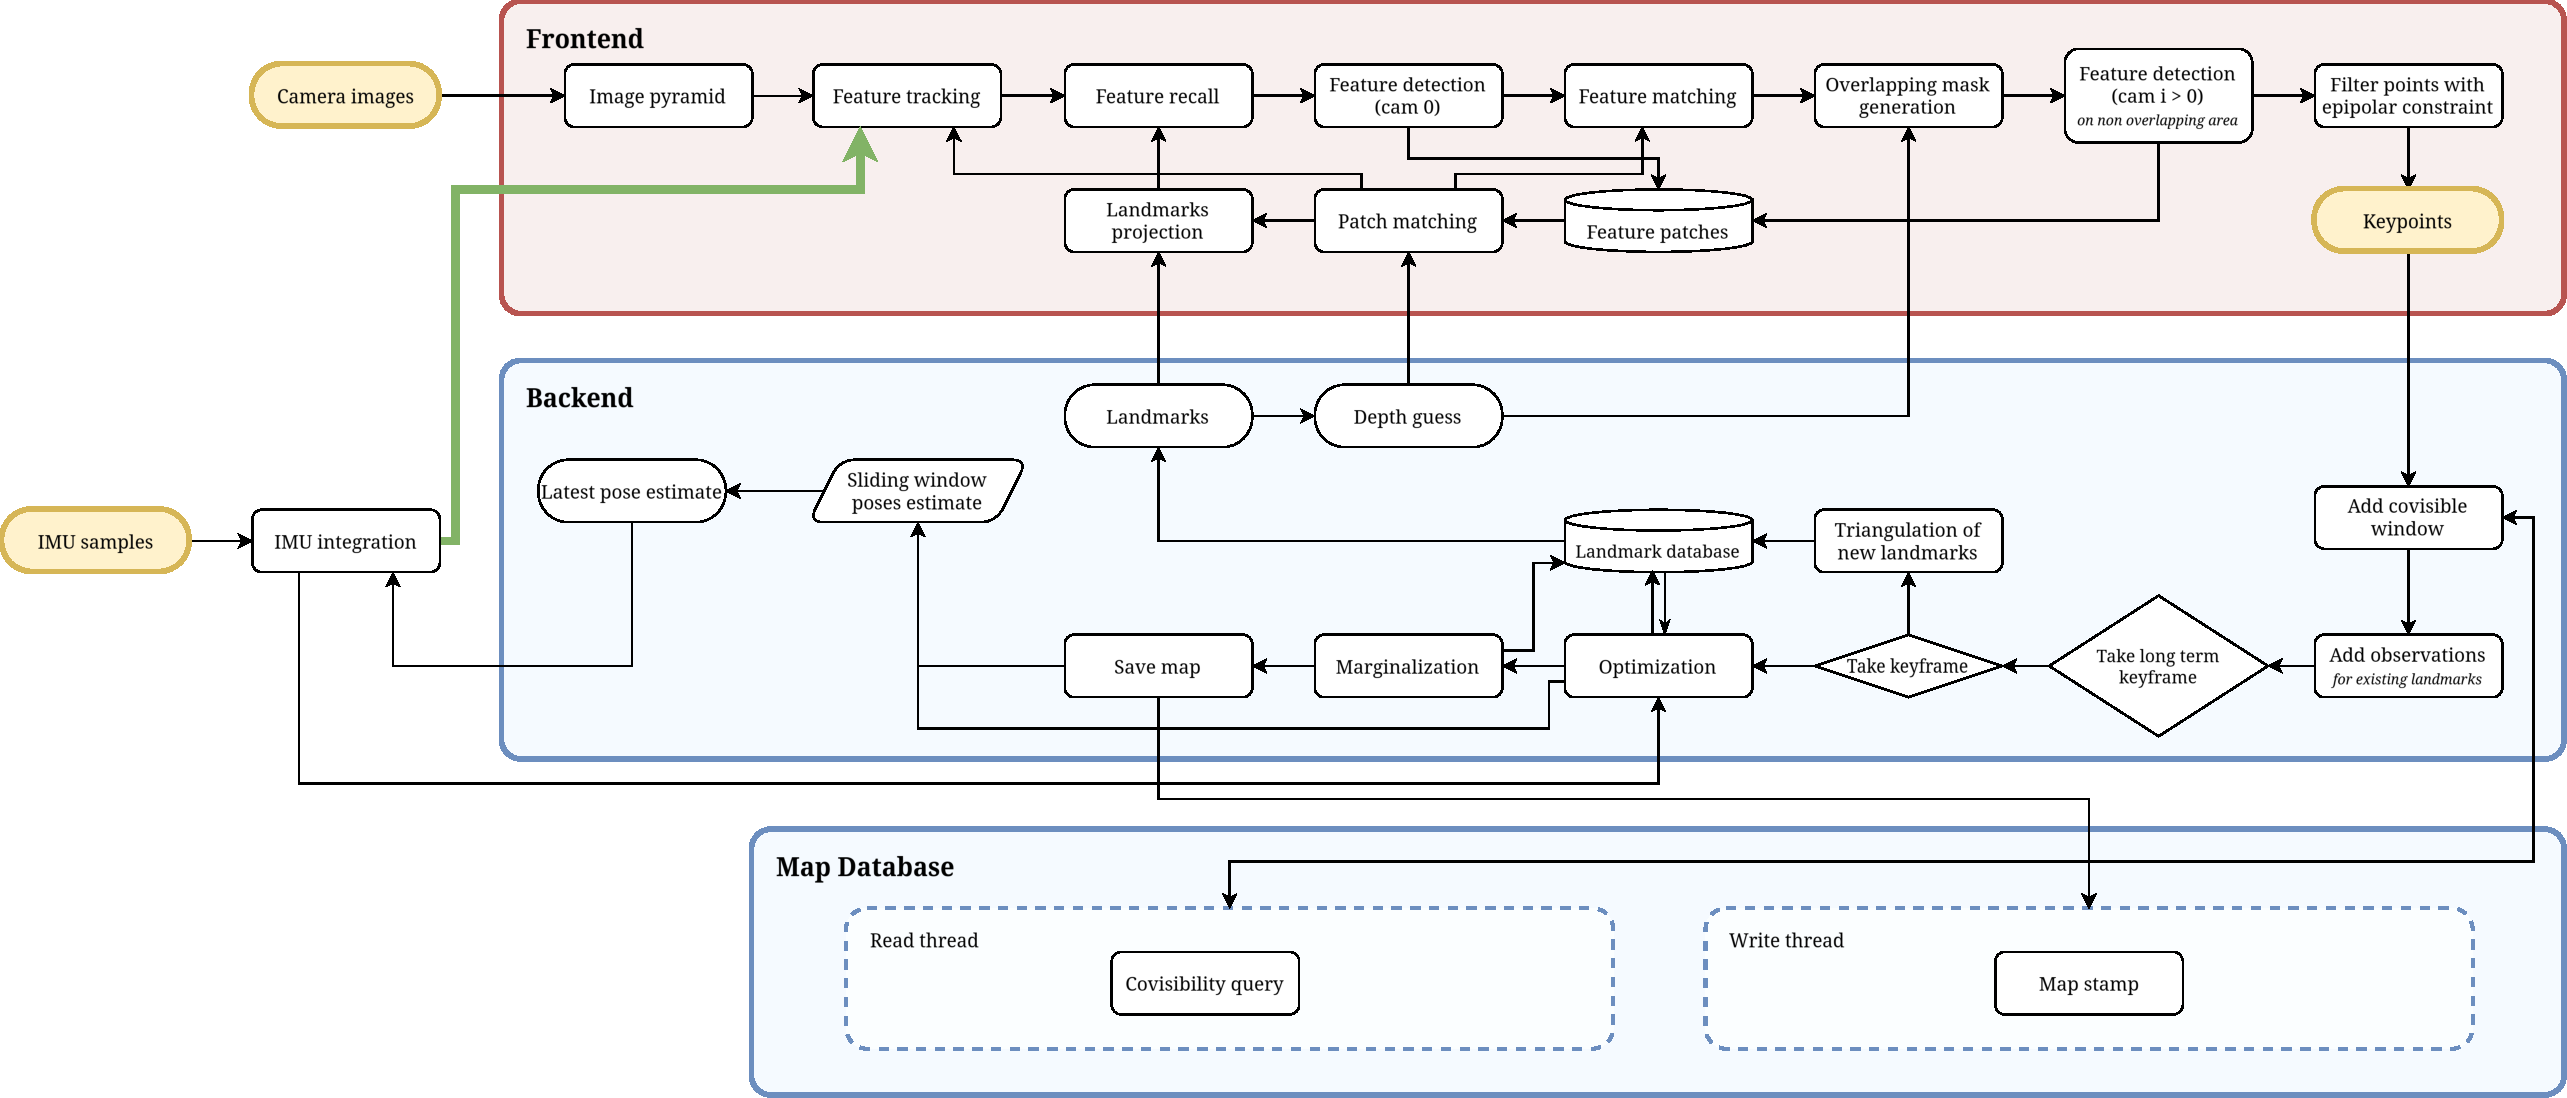
\includegraphics[width=0.9\linewidth]{img/method/arch.basaltxr.pdf}
    \caption{Arquitectura de Basalt-XR.}
    \label{fig:arch_basaltxr}
\end{figure}

\subsection{Front end}

Este hilo se encarga de procesar las imágenes capturadas por las cámaras, detectando y siguiendo los features a través de los frames.

Las imágenes ingresan al pipeline de Basalt a través del hilo del front-end. Inicialmente, se genera una representación piramidal de las imágenes, también conocidas como mipmaps, que consisten en múltiples copias de la misma imagen en diferentes resoluciones. Los mipmaps se utilizan ampliamente en el procesamiento de imágenes y visión por computadora para mejorar la eficiencia y robustez de los algoritmos frente a cambios de escala. Por ejemplo, en el cálculo del optical flow, los mipmaps se utilizan para manejar grandes movimientos de píxeles entre frames, calculando primero el movimiento en la resolución más baja y luego refinándolo en resoluciones más altas.

El hilo comienza con el tracking de los features detectados en el frame anterior. Para ello, Basalt está basado en optical flow, utilizando el algoritmo de Lucas-Kanade (KLT)~\cite{lucas1981klt} para el seguimiento de los features. Para ello, Basalt utiliza parches de 52 px por defecto. Para tener una buena estimación inicial (o prior) para el algoritmo, se utiliza la información de la IMU, que permite predecir la posición del keypoint en el siguiente frame a partir del movimiento de la cámara entre frames.

Una vez que se completa el tracking, se intentan recuperar los features que se hayan perdido debido a oclusiones o movimientos rápidos, en un proceso que se denomina \textit{recall}. Para ello, el front-end almacena el parche de cada keypoint detectado. Luego, proyecta los landmarks, que recibe del back-end, en el frame actual. Finalmente, intenta trackear cada uno de estos puntos con KLT, utilizando el parche almacenado y la proyección como prior. El funcionamiento del proceso se muestra en la Figura \ref{fig:recall_frames}, donde se observa la recuperación de un feature que se pierde debido a una oclusión de la cámara.

\begin{figure}[ht]
    \centering
    \begin{subfigure}[b]{0.32\textwidth}
        \centering
        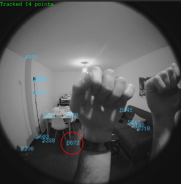
\includegraphics[width=\textwidth]{img/method/recall_964.png}
        \caption{Frame 964}
        \label{fig:recall_964}
    \end{subfigure}
    \hfill
    \begin{subfigure}[b]{0.32\textwidth}
        \centering
        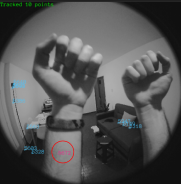
\includegraphics[width=\textwidth]{img/method/recall_982.png}
        \caption{Frame 982}
        \label{fig:recall_982}
    \end{subfigure}
    \hfill
    \begin{subfigure}[b]{0.32\textwidth}
        \centering
        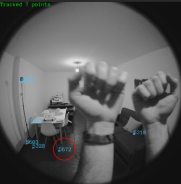
\includegraphics[width=\textwidth]{img/method/recall_1000.png}
        \caption{Frame 1000}
        \label{fig:recall_1000}
    \end{subfigure}
    \caption{Frames extraídos de la secuencia MIO02 del Monado SLAM Dataset ejecutada
    donde se observa la funcionalidad de recall. En (\subref{fig:recall_964}), el front-end de Basalt
    detecta un feature en la pata de la mesa con ID 5672 en el frame 964. En (\subref{fig:recall_982}) el
    seguimiento se pierde debido a una oclusión de la cámara, si embargo se intenta recuperar mediante
    la proyección del landmark (en rosa). Finalmente, en (\subref{fig:recall_1000}), se logra emparejar
    la proyección, reidentificando el feature exitosamente.}
    \label{fig:recall_frames}
\end{figure}

Una vez completados dichos procesos, que se basan en el seguimiento de los features, se realiza una detección de nuevos features utilizando el algoritmo FAST (Features from Accelerated Segment Test)~\cite{rosten2006fast}. Este algoritmo es un método eficiente para detectar esquinas en imágenes, lo que lo hace adecuado para aplicaciones en tiempo real como el SLAM.
%FAST funciona analizando un círculo de 16 píxeles alrededor de cada píxel candidato y clasificando el píxel como una esquina si un número suficiente de píxeles en el círculo son significativamente más brillantes o más oscuros que el píxel central. En la Figura \ref{fig:fast} se observa un parche de 16 px alrededor de un keypoint.
Un potencial problema del algoritmo es que los keypoints detectados pueden no estar bien distribuidos en la imagen, lo que puede resultar en una concentración en ciertas áreas de la imagen mientras que otras áreas quedan sin suficientes keypoints. Para mitigar este problema, Basalt divide el frame en celdas (de 50 x 50 px por defecto), en donde se detectan los nuevos keypoints. Por celda, solo se conserva el keypoint de mejor calidad. Además, en aquellas celdas donde ya hay features trackeados, no se realiza la detección de nuevos keypoints. En el caso ideal, solo será necesario detectar keypoints en porciones de la imagen donde se observe una nueva escena.

%\begin{figure}[h]
%    \centering
%    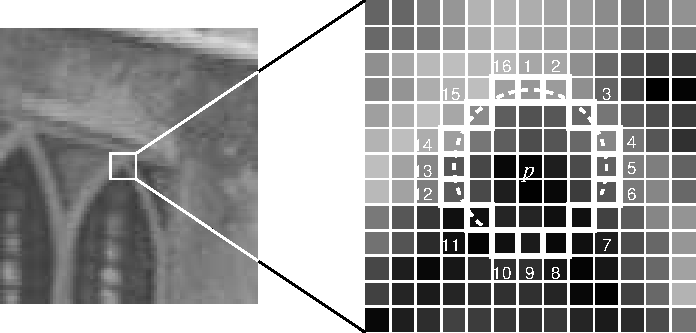
\includegraphics[width=0.8\linewidth]{img/method/FAST.pdf}
%    \caption{Imagen extraída del paper de FAST [10] donde se representa la detección de features
%    mediante un parche de 16 píxeles.}
%    \label{fig:fast}
%\end{figure}

A continuación, se generan máscaras en las zonas superpuestas de las cámaras secundarias con la principal, con el objetivo de buscar correspondencias (matching) entre los keypoints de las cámaras. Para lograr esto, se aplica el mismo proceso de seguimiento de features utilizando KLT, pero en lugar de realizarse entre frames capturados en diferentes timestamps, se realiza entre frames capturados simultáneamente por las dos cámaras.
Como el sistema debe funcionar en configuraciones de cámaras no paralelas, se utiliza un algoritmo que predice la posición de un keypoint en la cámara secundaria a partir de su posición en la cámara principal, utilizando una estimación de la profundidad de la escena que realiza el back-end. Finalmente, se realiza una segunda detección de keypoints en las áreas no superpuestas, para asegurar que se detecten suficientes keypoints en toda la imagen. Este proceso se muestra en la Figura \ref{fig:frontend_detection_process}.

\begin{figure}[ht]
    \centering
    \begin{subfigure}[b]{0.48\textwidth}
        \centering
        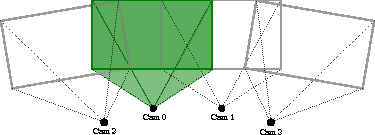
\includegraphics[width=\textwidth]{img/method/detection_1.pdf}
        \caption{Detección en cámara principal}
        \label{fig:frontend_detection_process_a}
    \end{subfigure}
    \hfill
    \begin{subfigure}[b]{0.48\textwidth}
        \centering
        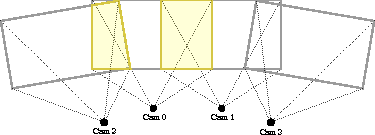
\includegraphics[width=\textwidth]{img/method/detection_2.pdf}
        \caption{Generación de máscaras}
        \label{fig:frontend_detection_process_b}
    \end{subfigure}

    \vspace{0.5em}

    \begin{subfigure}[b]{0.48\textwidth}
        \centering
        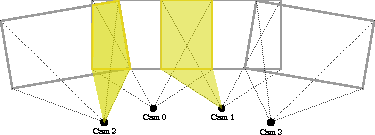
\includegraphics[width=\textwidth]{img/method/detection_3.pdf}
        \caption{Matching multicámara}
        \label{fig:frontend_detection_process_c}
    \end{subfigure}
    \hfill
    \begin{subfigure}[b]{0.48\textwidth}
        \centering
        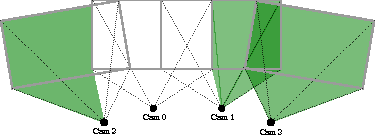
\includegraphics[width=\textwidth]{img/method/detection_4.pdf}
        \caption{Detección en áreas no superpuestas}
        \label{fig:frontend_detection_process_d}
    \end{subfigure}

    \caption{Proceso de detección del front-end luego de la mejora de soporte para múltiples cámaras. En primer lugar, se detectan features en la cámara principal (\subref{fig:frontend_detection_process_a}), luego se generan las máscaras para ignorar zonas superpuestas (\subref{fig:frontend_detection_process_b}) y se realiza el matching multicámaras (\subref{fig:frontend_detection_process_c}). Finalmente, se realiza una segunda detección en las áreas no superpuestas (\subref{fig:frontend_detection_process_d}).}
    \label{fig:frontend_detection_process}
\end{figure}

%\begin{figure}[h]
%    \centering
%    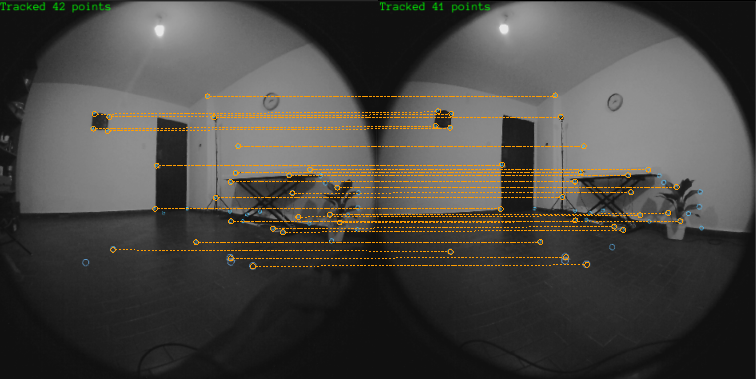
\includegraphics[width=0.8\linewidth]{img/method/matching.pdf}
%    \caption{Ejemplo del proceso de matching estéreo.}
%    \label{fig:matching}
%\end{figure}

Finalmente, se realiza un filtrado de matches empleando la restricción epipolar, ilustrado en la Figura~\ref{fig:epipolar_geometry}. Para cada par de observaciones 2D del mismo keypoint en dos cámaras, se desprojectan ambas posiciones a rayos normalizados en coordenadas de cámara. Luego se evalúa el error epipolar algebraico como $|{\mathbf{x}_l}^\top \mathbf{E} \, \mathbf{x}_r|$, donde $\mathbf{x}_l$ y $\mathbf{x}_r$ son dichos rayos y $\mathbf{E}$ es la matriz esencial entre el par de cámaras. Esta expresión cuantifica, para una correspondencia, cuánto se aleja de la condición de coplanaridad del plano epipolar. Si este error supera un umbral predefinido, la correspondencia es descartada.

\begin{figure}[h]
    \centering
    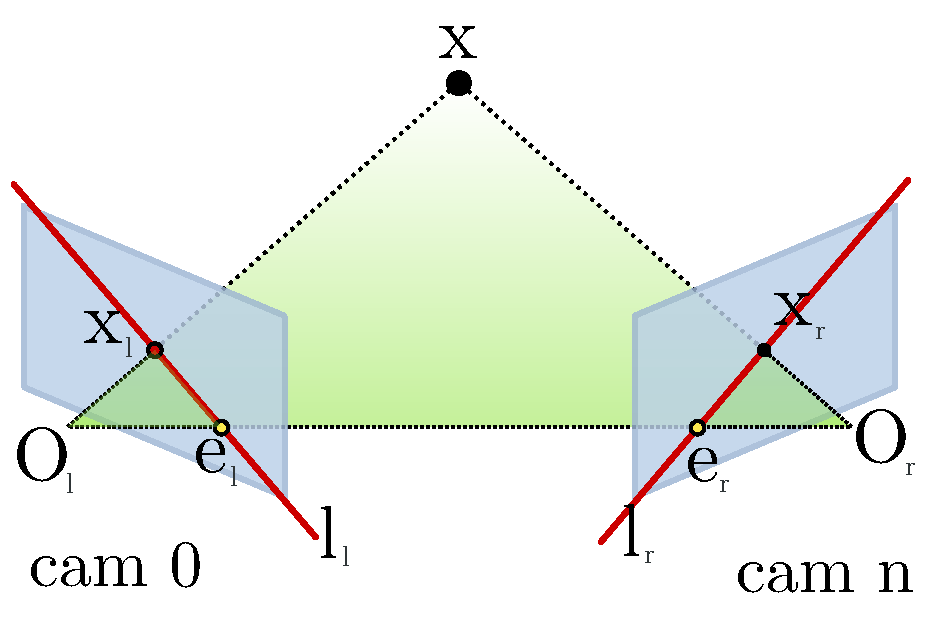
\includegraphics[width=0.5\linewidth]{img/method/epipolar_geometry.pdf}
    \caption{Geometría epipolar. El punto $\mathbf{X}$ es observado desde dos cámaras con centros ópticos $\mathbf{O}_l$ y $\mathbf{O}_r$, proyectándose en $\mathbf{x}_l$ y $\mathbf{x}_r$ respectivamente. Los tres puntos $\mathbf{O}_l$, $\mathbf{O}_r$ y $\mathbf{X}$ definen el plano epipolar, cuya intersección con cada imagen forma las líneas epipolares $\mathbf{l}_l$ y $\mathbf{l}_r$. Los puntos $\mathbf{e}_l$ y $\mathbf{e}_r$ son los epípolos, es decir, las proyecciones de cada centro óptico en la imagen opuesta.}
    \label{fig:epipolar_geometry}
\end{figure}

\subsection{Back end}

El back-end de Basalt-XR se ejecuta en hilos paralelos al front end. Consta de dos componentes principales que ejecutan en threads separados: el VIO y el mapa persistente (MapDatabase). El primero recibe como entradas las mediciones de la IMU y los resultados del optical flow, es decir, los keypoints detectados en cada frame. Su objetivo principal es realizar una estimación precisa de una ventana local de keyframes, frames y landmarks. El segundo componente, el mapa persistente, se encarga de almacenar la información de los keyframes y landmarks a largo plazo. Esto lo convierte en un sistema VI-SLAM, que le permite aumentar significativamente la precisión, a través de operaciones como la reintroducción de keyframes covisibles a la ventana local, la detección y cierre de ciclos, o la ejecución de optimizaciones globales.

\subsubsection{VIO}

El VIO mantiene una ventana local de keyframes, frames y landmarks que se optimiza continuamente, y se encuentra almacenada en una clase denominada \texttt{LandmarkDatabase} (véase Figura~\ref{fi:vio_window}). En primer lugar, el VIO integra las mediciones de la IMU utilizando un filtro de preintegración, dado que la frecuencia de la IMU es típicamente mucho mayor que la de las cámaras. Luego, se realiza opcionalmente una consulta de covisibilidad al mapa persistente, para reintroducir keyframes y landmarks previamente marginalizados en la ventana de optimización local. Existen diferentes estrategias para que el mapa resuelva estas consultas, que se detallarán más adelante. Estos keyframes se introducen temporalmente, hasta la próxima consulta. Esta funcionalidad se debe combinar con el recall, de modo que los keyframes reintroducidos sirvan para volver a trackear keypoints que se hayan perdido en el front-end y así obtener observaciones que relacionen los keyframes reintroducidos con los frames más recientes.

\begin{figure}[h]
    \centering
    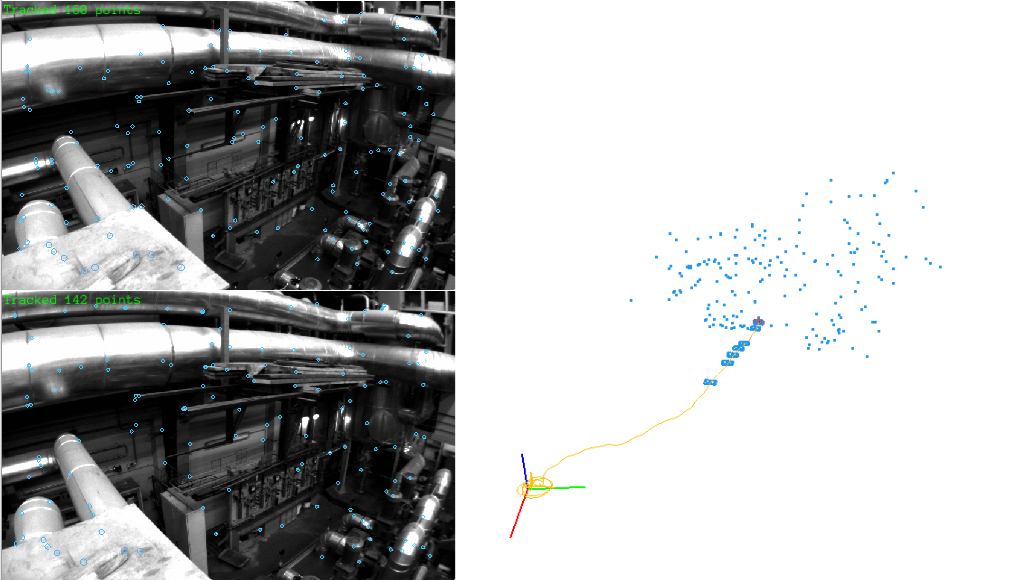
\includegraphics[width=0.5\linewidth]{img/method/vio.png}
    \caption{Captura de pantalla de la ventana local de keyframes y landmarks del VIO.}
    \label{fig:vio_window}
\end{figure}

A continuación, se predice la pose del frame actual propagando las mediciones pre-integradas de la IMU desde la pose del frame anterior, y se registran las observaciones de los keypoints que el front-end detectó y el VIO había triangulado previamente. Finalmente, se evalúa si el frame actual debe promoverse a keyframe, decisión que se toma mediante una heurística basada en dos criterios: (1) la proporción de keypoints del frame actual con correspondencias en otros keyframes de la ventana, respecto del total de keypoints detectados; y (2) la cantidad de frames transcurridos desde el último keyframe.

Si se decide tomar un nuevo keyframe, se triangula la posición tridimensional de aquellos keypoints cuyas observaciones aún no están conectadas con la ventana. Para ello, es necesario contar con una segunda observación del landmark en alguno de los frames posteriores al último keyframe. Para cada observación $z_{ih} \in \mathbb{R}^2$ del landmark $i$ en el keyframe actual $h$, al que se denomina host, se recorren los frames desde el keyframe anterior en búsqueda de una segunda observación $z_{it} \in \mathbb{R}^2$ del mismo landmark en algún frame target $t$. En caso de hallarse, la triangulación procede de la siguiente manera:
\begin{enumerate}
    \item Se calcula la transformación relativa entre la cámara que observa el punto en el frame host y la cámara que lo observa en el frame target, utilizando las poses estimadas de ambos frames.
    \item Si la distancia entre ambas cámaras es menor a un umbral predefinido, se descarta la triangulación, y se procede a buscar otro frame target.
    \item Se desproyectan ambas observaciones a rayos normalizados en coordenadas de cámara.
    \item Se calcula la posición tridimensional del landmark a partir de los rayos y la transformación relativa entre las cámaras, según lo descrito por Hartley y Zisserman~\cite{hartley2004multipleviewgeometry} en el Capítulo 12.
\end{enumerate}

El resultado de la triangulación es un vector de $\mathbb{R}^4$ en coordenadas homogéneas, donde los primeros tres elementos representan el vector unitario o bearing vector que determina la dirección desde el frame host al landmark y el cuarto corresponde a la distancia inversa. Luego, se utiliza la proyección estereográfica para representar el bearing vector en 2 dimensiones. La posición de cada landmark se almacena en la clase \texttt{LandmarkDatabase}, y queda ligada a la pose del keyframe host.

Luego de procesar un frame, Basalt optimiza el estado del sistema $s = \{s_k, s_f, s_l\}$, donde $s_k$ son las poses de los keyframes de la ventana, $s_f$ las poses, velocidades y biases de los frames más recientes, y $s_l$ los landmarks de la ventana. Modela las relaciones entre variables con un grafo de factores, y mediante mínimos cuadrados no lineales con Levenberg-Marquardt, minimiza la función de energía:
\begin{align}
E = E_L + E_I + E_m
  &= \sum_{\substack{i \in L \\ t \in \text{obs}(i)}} r_{it}^\top \Sigma_{it}^{-1} r_{it}
   + \sum_{(i,j) \in C} r_{ij}^\top \Sigma_{ij}^{-1} r_{ij} + E_m,
\end{align}
donde $E_L$ agrega los residuales de reproyección de landmarks, $E_I$ los de preintegración de la IMU y $E_m$ un prior de marginalización.

Luego de la optimización, Basalt marginaliza variables del estado para mantener el sistema acotado en tamaño. El proceso determina qué variables eliminar según dos criterios: si hay más de 7 keyframes, se marginaliza aquel cuya proporción de landmarks hosteados que fueron observados en la ventana sea menor a un umbral, o en su defecto el más cercano espacialmente al resto (el más redundante). Adicionalmente, en toda iteración se marginaliza el frame más antiguo, eliminando velocidad y biases, conservando su pose únicamente si fue seleccionado como keyframe.

Antes de descartar definitivamente esas variables, se calcula un prior de marginalización que condensa su información en dos matrices $H$ y $b$. Estas matrices se incorporan a la optimización de la siguiente iteración como un término adicional de marginalización, garantizando que la información de las variables eliminadas siga influyendo en el sistema. Finalmente, las poses, frames y landmarks marginalizados se eliminan del estado y de la \texttt{LandmarkDatabase}.

\begin{figure}[ht]
    \centering
    \begin{subfigure}[b]{0.32\textwidth}
        \centering
        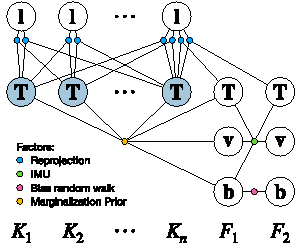
\includegraphics[width=\textwidth]{img/method/basalt.state1.pdf}
        \caption{}
        \label{fig:basalt_state_a}
    \end{subfigure}
    \hfill
    \begin{subfigure}[b]{0.32\textwidth}
        \centering
        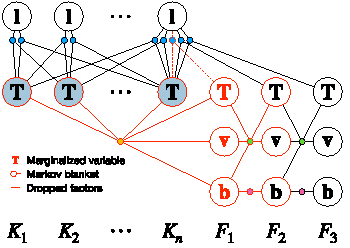
\includegraphics[width=\textwidth]{img/method/basalt.state2.pdf}
        \caption{}
        \label{fig:basalt_state_b}
    \end{subfigure}
    \hfill
    \begin{subfigure}[b]{0.32\textwidth}
        \centering
        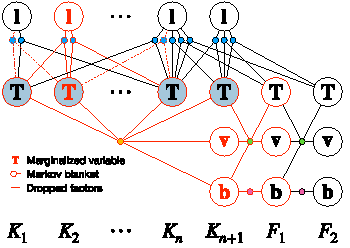
\includegraphics[width=\textwidth]{img/method/basalt.state3.pdf}
        \caption{}
        \label{fig:basalt_state_c}
    \end{subfigure}

    \caption{Grafo de factores de Basalt. (\subref{fig:basalt_state_a}) después de marginalizar un frame, el sistema está compuesto por los últimos $n$ keyframes $K_1 \dots K_n$ y los $m - 1$ frames más recientes, $F_1$ y $F_2$ (en este ejemplo, el sistema trabaja con un máximo de 3 frames). Cuando llega un nuevo frame ($F_3$), se marginaliza el frame más antiguo ($F_1$), y se pueden dar dos escenarios. En el primero~(\subref{fig:basalt_state_b}), si $F_1$ no se convierte en un keyframe, el frame completo es marginalizado, eliminando bias, velocidad y pose. En el segundo~(\subref{fig:basalt_state_c}), si $F_1$ es promovido a keyframe, solo se marginalizan sus variables de bias y velocidad, a la vez que otro keyframe es seleccionado para ser marginalizado.}
    \label{fig:basalt_state}
\end{figure}

Antes de pasar al siguiente frame, el thread envía al front-end la estimación del estado, los landmarks de la ventana local y la profundidad promedio de la escena. Asimismo, envía al mapa persistente una copia de la \texttt{LandmarkDatabase} encapsulada en una estructura \texttt{MapStamp}, para que este pueda actualizar su información a largo plazo.

\subsubsection{Mapa persistente}

Este mapa persistente almacena la información de keyframes y landmarks una vez que han sido optimizados por la capa del VIO. Fue diseñado para actualizarse de forma continua a medida que se exploran nuevas zonas y, simultáneamente, para permitir realizar consultas que reutilicen esa información de manera inteligente (véase Figura~\ref{fig:persistent_map}).

\begin{figure}[ht]
    \centering
    \begin{subfigure}[b]{0.4\textwidth}
        \centering
        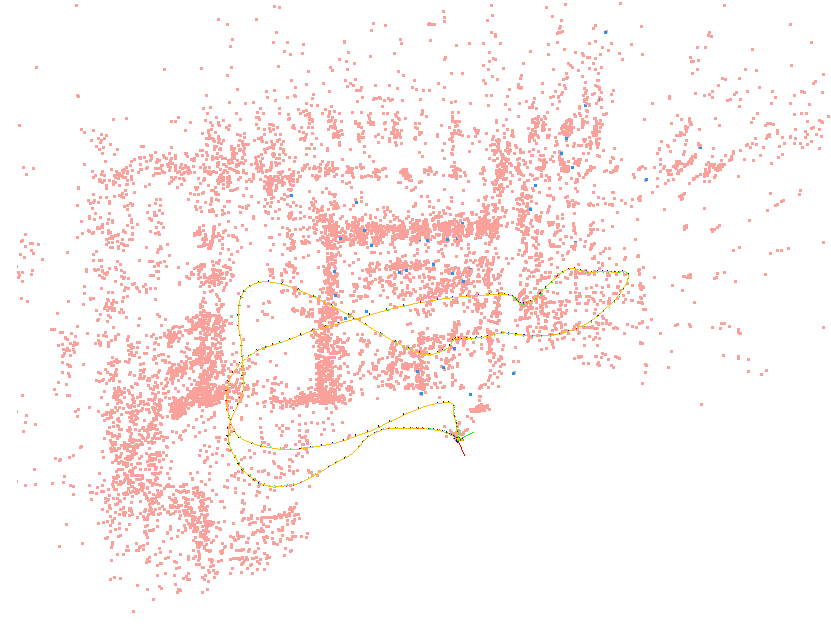
\includegraphics[width=\textwidth]{img/method/persistent.map.png}
        \caption{}
        \label{fig:persistent_map_cenital}
    \end{subfigure}
    \hspace{2em}
    \begin{subfigure}[b]{0.4\textwidth}
        \centering
        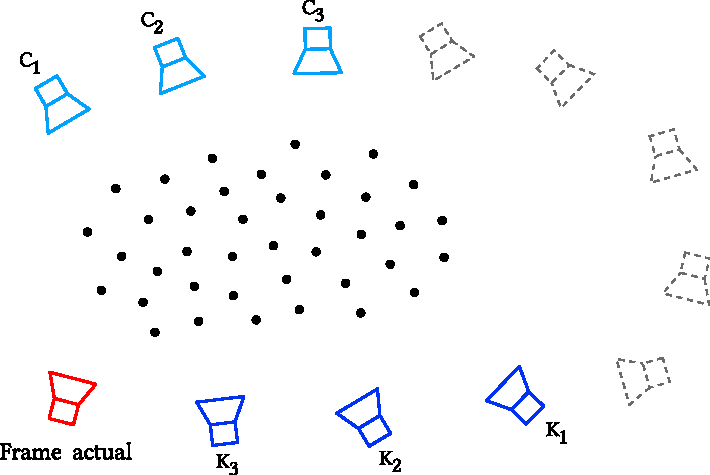
\includegraphics[width=\textwidth]{img/method/covisibility.pdf}
        \caption{}
        \label{fig:persistent_map_covisibility}
    \end{subfigure}

    \caption{Mapa persistente. En (\subref{fig:persistent_map_cenital}) una vista cenital del mapa persistente, con los landmarks en rosa y las poses de los keyframes a lo largo de la trayectoria. En (\subref{fig:persistent_map_covisibility}) un diagrama que ilustra la introducción de keyframes $C_1$, $C_2$ y $C_3$ del mapa, a la ventana local, mediante la consulta de covisibilidad.}
    \label{fig:persistent_map}
\end{figure}

La implementación del mapa persistente se encuentra en la clase \texttt{MapDatabase}, responsable de inicializarlo, actualizarlo, gestionar consultas y manejar el acceso de lectura y escritura. Para almacenar la información del mapa, se reutiliza la clase \texttt{LandmarkDatabase}, ya empleada por el VIO para representar la ventana de keyframes. Una ventaja clave de este diseño es su capacidad de funcionar de manera asíncrona: otros componentes del sistema, como el VIO, interactúan con el mapa a través de colas de trabajo sin bloquear su ejecución.

Al iniciarse, se crean dos subprocesos principales: \texttt{reading\_thread} y \texttt{writing\_thread}. El primero procesa las consultas de lectura al mapa, siendo la consulta de covisibilidad la única funcionalidad implementada de este tipo. El segundo procesa las consultas de escritura, donde la única operación implementada es la actualización del mapa mediante el \texttt{MapStamp}. Para garantizar la consistencia de los datos, ambos subprocesos comparten un mecanismo de bloqueo mediante mutex que regula el acceso concurrente al mapa, evitando condiciones de carrera.

Se implementaron dos estrategias para resolver la consulta de covisibilidad:
\begin{itemize}
    \item Covisibilidad por observaciones: La ventana de covisibilidad se compone del último keyframe introducido en el mapa junto con todos aquellos keyframes que observen al menos un landmark en común con este. Además, se incluyen todos los landmarks cuyo host se encuentre entre esos keyframes.
    \item Covisibilidad espacial: Esta estrategia selecciona keyframes que observan la misma región del espacio que el keyframe más reciente, siguiendo el enfoque presentado en~\cite{peng2021reidentification}. Para cada keyframe se construye un cubo tridimensional (\textit{spatial distribution cube}) centrado en la media de las posiciones 3D de sus landmarks, con extensión proporcional a la varianza de esas posiciones en cada eje. Ante una consulta del VIO, se devuelven los keyframes cuyos cubos se solapan con el del keyframe más reciente, priorizando los más antiguos para minimizar el drift acumulado, junto con todos los landmarks hosteados por ellos. La cantidad total de keyframes devueltos se limita mediante un parámetro configurable del sistema.
\end{itemize}

\section{Cierre de ciclos}

A partir del sistema descrito en la sección anterior, se propone la implementación de un módulo de cierre de ciclos capaz de detectar y corregir los errores acumulados en la estimación de la trayectoria a largo plazo. Para ello, se incorpora al back-end un nuevo thread denominado \texttt{LoopClosing}, que opera en paralelo al VIO y al mapa persistente. El proceso comprende tres etapas: detección, optimización del grafo de poses (PGO) y fusión de mapa. La Figura~\ref{fig:arch_basaltslam} muestra la arquitectura del sistema resultante.

% TODO: de esta figura, eliminar el componente de RootBA
\begin{figure}[h]
    \centering
    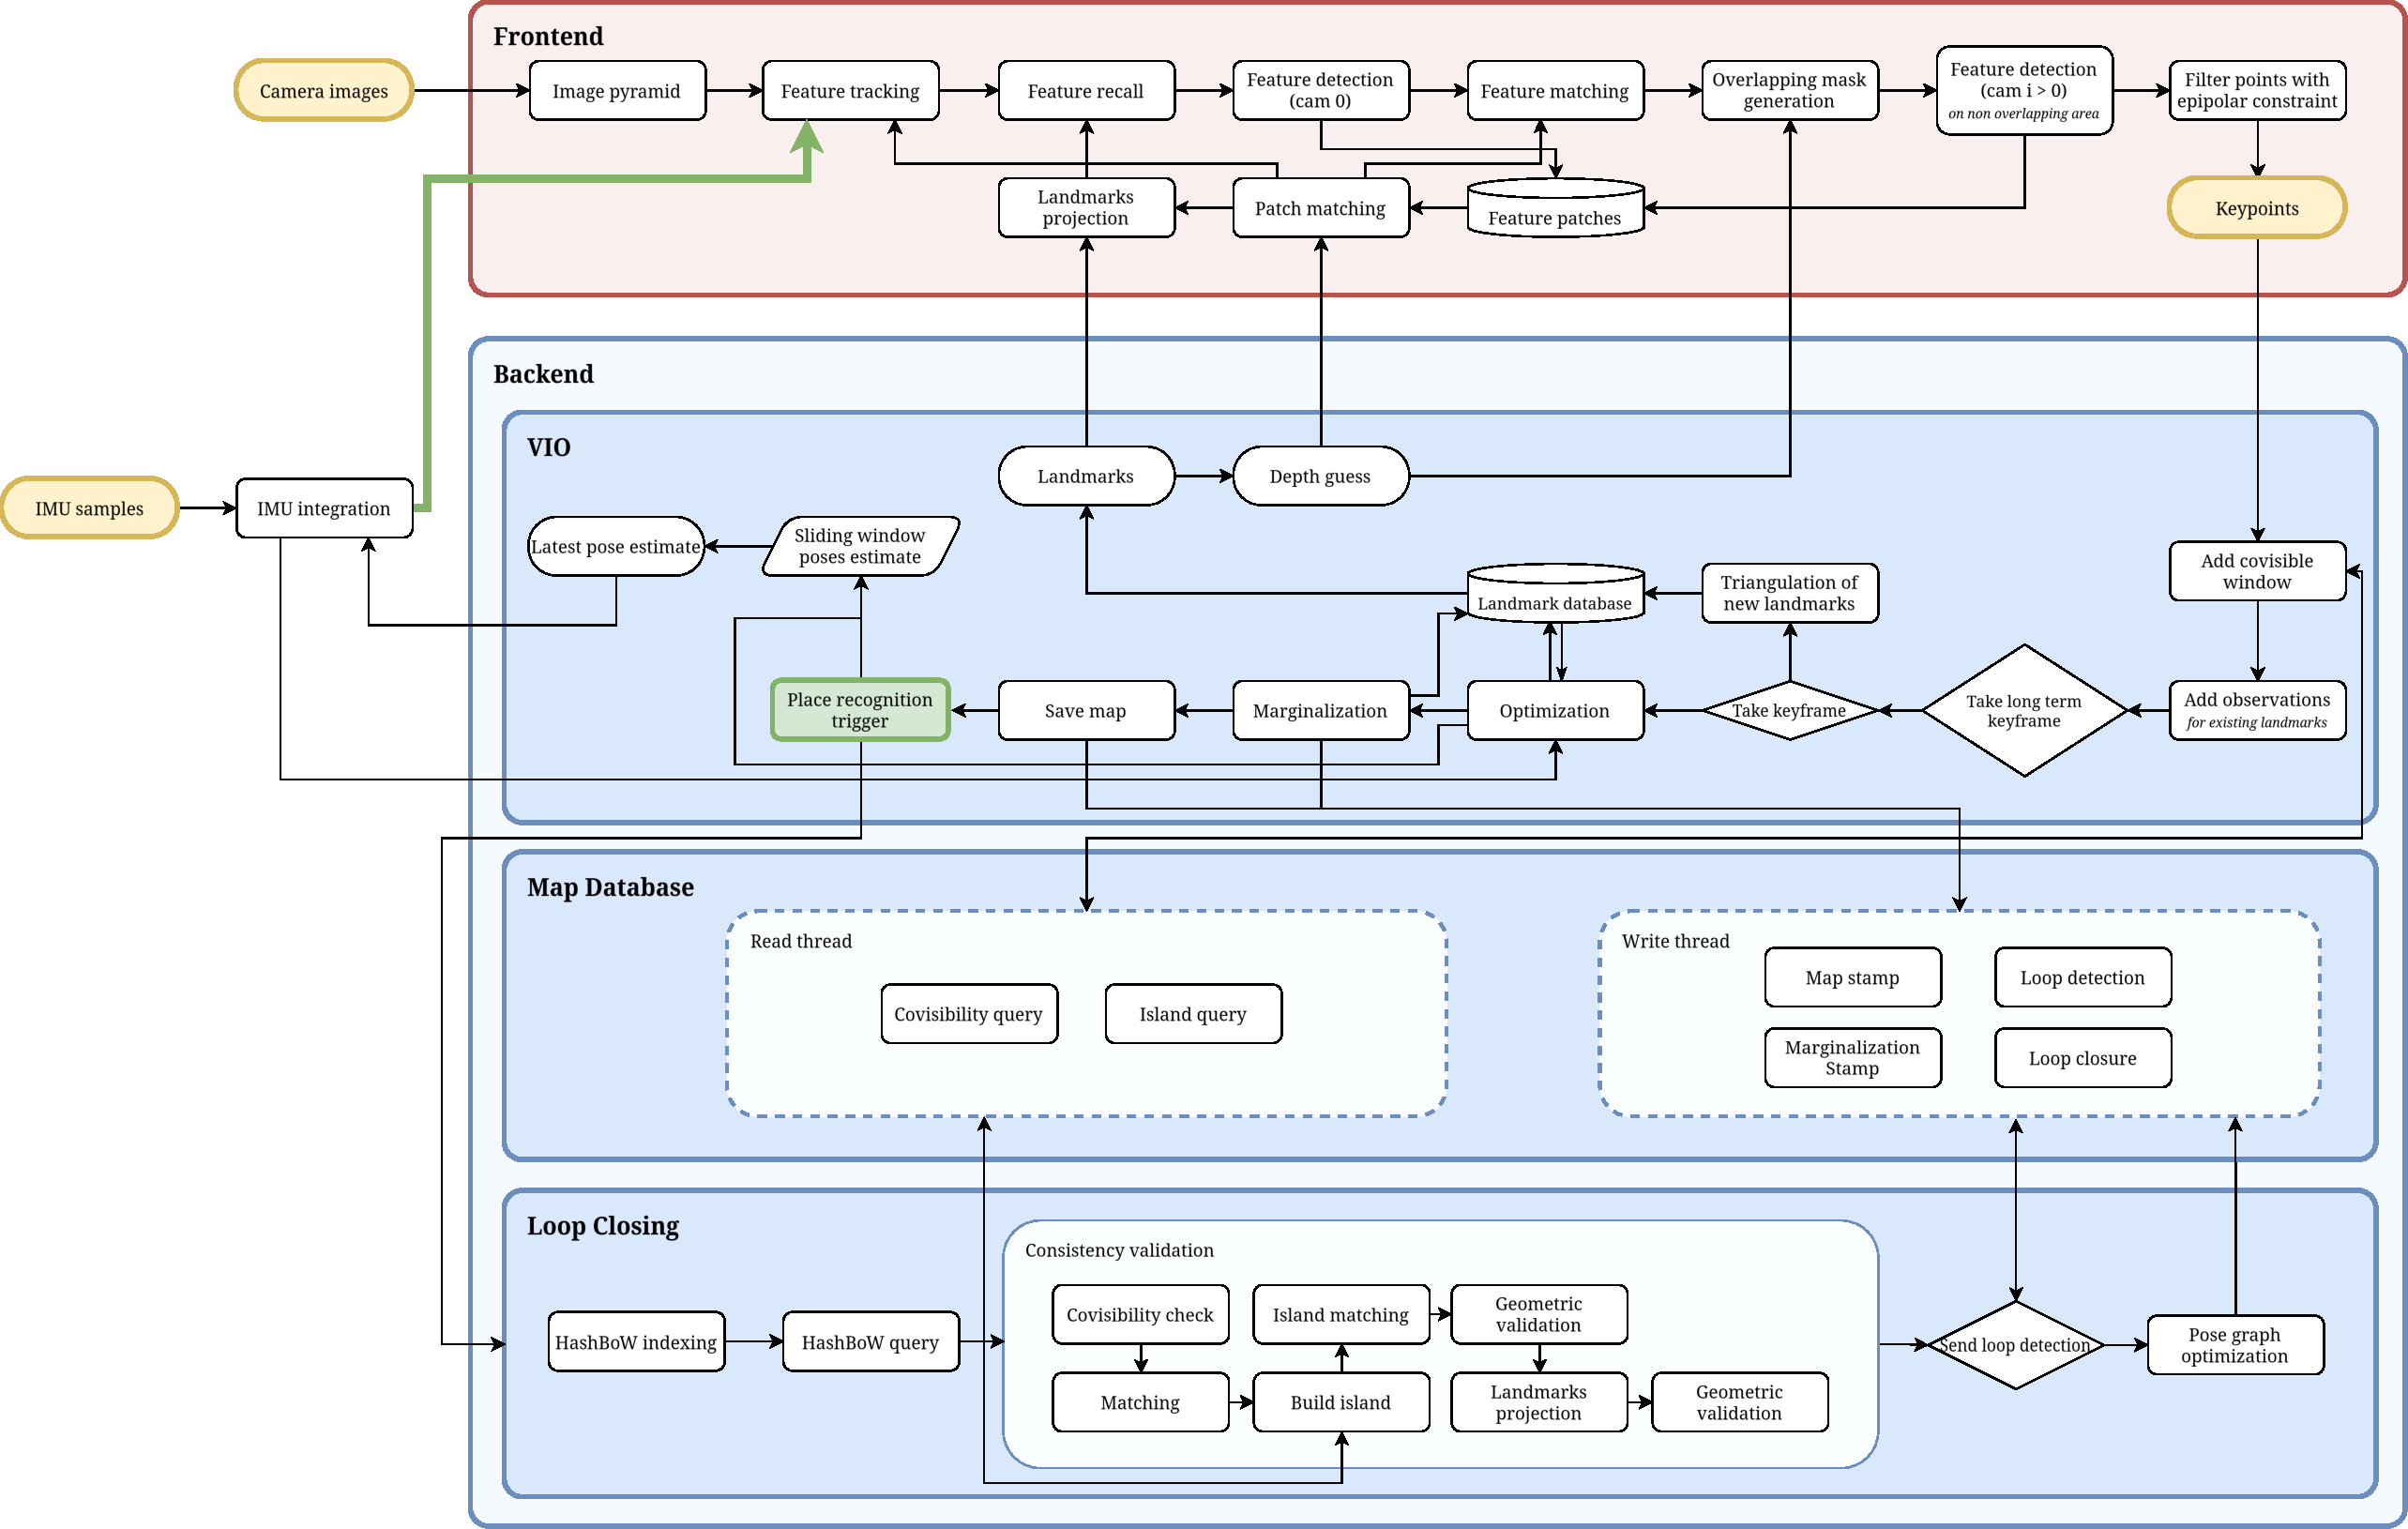
\includegraphics[width=0.9\linewidth]{img/method/arch.loopclosure.pdf}
    \caption{Arquitectura del sistema propuesto, con la incorporación del thread \texttt{LoopClosing}.}
    \label{fig:arch_basaltslam}
\end{figure}

La Figura~\ref{fig:loop_decision} resume el flujo de comunicación entre \texttt{LoopClosing} y \texttt{MapDatabase}. Ante la detección de un ciclo, el mapa persistente evalúa si el drift acumulado es suficiente para justificar una corrección. De ser así, envía al thread \texttt{LoopClosing} un puntero a una copia liviana del mapa con las poses de los keyframes, junto con las aristas del grafo de poses necesarias para optimizar la trayectoria mediante PGO. Las poses optimizadas resultantes se devuelven al mapa persistente para su aplicación. De lo contrario, el mapa notifica al thread que la optimización no procederá, permitiéndole continuar su ejecución. En ambos casos, para el mapa persistente, el proceso finaliza con la etapa de fusión de mapa.

\begin{figure}[ht]
    \centering
    \begin{subfigure}[b]{0.36\textwidth}
        \centering
        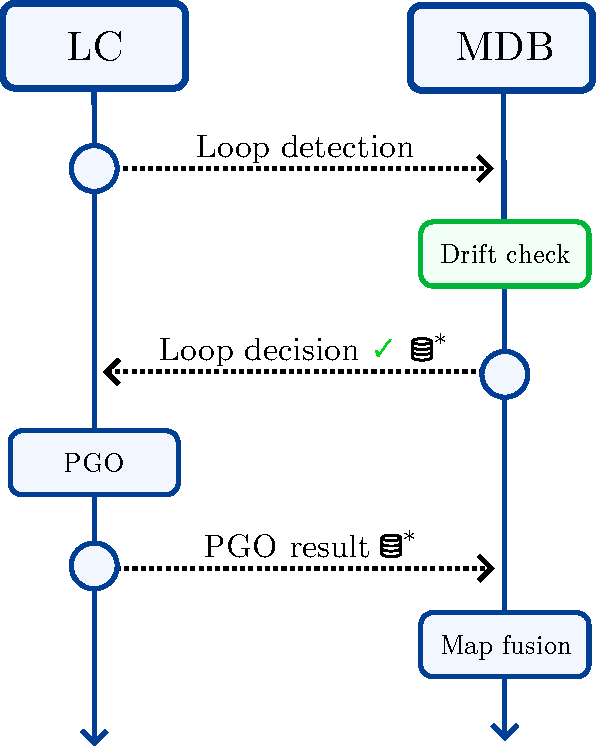
\includegraphics[width=\textwidth]{img/method/loop_decision_ok.pdf}
        \caption{Detección con suficiente drift.}
        \label{fig:loop_decision_ok}
    \end{subfigure}
    \hspace{4em}
    \begin{subfigure}[b]{0.36\textwidth}
        \centering
        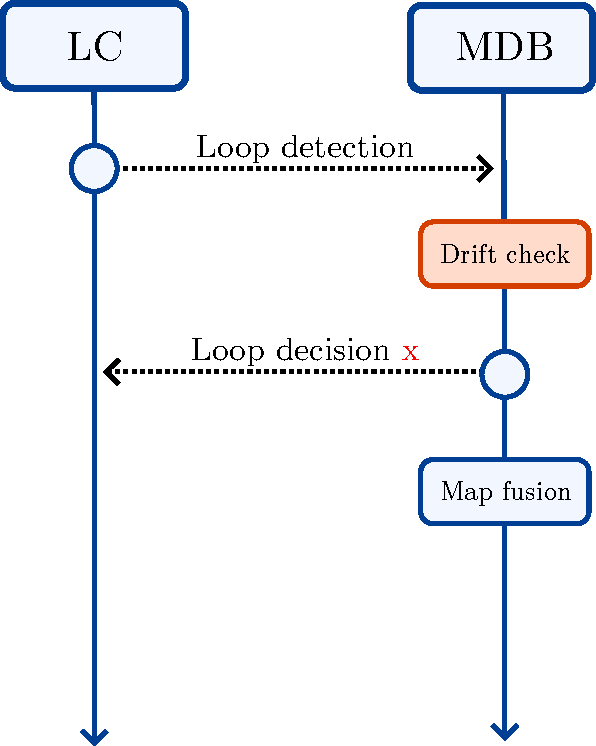
\includegraphics[width=\textwidth]{img/method/loop_decision_rej.pdf}
        \caption{Detección con drift insuficiente.}
        \label{fig:loop_decision_rej}
    \end{subfigure}
    \caption{Comunicación entre \texttt{LoopClosing} y \texttt{MapDatabase} según el drift detectado.}
    \label{fig:loop_decision}
\end{figure}

\subsection{Detección de ciclos}

La detección de ciclos consiste en reconocer cuándo el sistema vuelve a observar una escena previamente visitada. Los métodos de \textit{place recognition} suelen basarse en descriptores visuales globales; en este trabajo se adopta un enfoque de Bag of Words (BoW), aprovechando los keypoints ya detectados por el front-end. En particular, se emplea el método HashBoW por su eficiencia computacional frente a otras alternativas, junto con descriptores locales binarios ORB, que ofrecen velocidad, robustez e invarianza ante rotaciones.

Se utiliza una configuración de HashBoW con 16 bits y vocabulario aleatorio, prescindiendo de entrenamiento previo. Esta decisión obedece a que un sistema de SLAM debe operar en entornos arbitrarios, lo que requeriría un vocabulario excesivamente general para ser útil; por ello se opta directamente por uno aleatorio. La similitud entre vectores BoW se mide mediante la norma $L_1$, y cada consulta devuelve los 10 keyframes más similares. Si bien se introducen una cantidad elevada de falsos positivos por las razones expuestas en la Sección~\ref{sec:hashbow}, el efecto se mitiga mediante una serie de verificaciones de consistencia adicionales descritas a continuación.

% The weighting type is a simple term frequency scheme. And the chosen similarity score between two BoW vectors is the L1 score (based on the L1 norm).

Como se observa en la Figura~\ref{fig:arch_basaltslam}, el proceso comienza cuando el VIO selecciona un keyframe y, tras enviar el \texttt{MapStamp} al mapa persistente, envía sus imágenes y los keypoints detectados al thread \texttt{LoopClosing}. Al recibirlos, se computan y almacenan los descriptores ORB de cada keypoint, se calcula un vector BoW por cámara a partir de dichos descriptores y se indexan en la HashBoW. Seguidamente, se consulta esta estructura con el vector de la cámara izquierda para obtener los candidatos, sobre los que se itera secuencialmente. El primer candidato que supere todas las verificaciones se selecciona para el cierre de ciclo.

Las verificaciones que se realizan sobre cada keyframe candidato $k_c$, en orden, son las siguientes (donde $k_r$ denota el keyframe más reciente): % a esto de k_r mencionarlo en otro lado tal vez, o mejor redactado
\begin{enumerate}
    \item Verificación de covisibilidad. Se comprueba que $k_r$ no comparta ninguna observación con $k_c$. De compartirlas, ambos keyframes estarían observando la misma escena sin drift acumulado, con lo que no habría ciclo que corregir.
    \item Correspondencias iniciales. Dado que este proceso se ejecuta para cada uno de los 10 candidatos, se realiza primero una búsqueda rápida de correspondencias mediante descriptores ORB. Si el número de matches es insuficiente, el candidato se descarta de forma temprana.
    \item Consulta de isla de candidatos (ver Figura~\ref{fig:candidates_island}). Se consulta al mapa persistente para obtener el conjunto de cuatro keyframes más covisibles con $k_c$, junto con todos los landmarks 3D observados por ellos. Este conjunto se denomina isla de candidatos.
    \item Correspondencias con la isla de candidatos. Se buscan correspondencias entre los descriptores ORB de los keypoints de $k_r$ y los de los landmarks 3D observados por la isla de candidatos. En este paso se exige un umbral de matches más alto para considerar válido al candidato.
    \item Verificación geométrica. Se estima la pose absoluta no-central de $k_r$ a partir de correspondencias 3D-2D entre los landmarks de la isla de candidatos y los keypoints de $k_r$. Para ello se emplea el algoritmo gP3P de OpenGV dentro de un esquema RANSAC. La estimación resultante se refina mediante mínimos cuadrados no lineales, minimizando el error de reproyección angular sobre el conjunto de inliers. Si no se halla una transformación válida, o si el número o la proporción de inliers no supera umbrales establecidos, el candidato se descarta.
    \item Proyección de landmarks (ver Figura~\ref{fig:reprojection_search}). Con el fin de ampliar el conjunto de correspondencias y obtener una estimación de la pose de $k_r$ más precisa y robusta, se proyectan sobre él los landmarks de la isla de candidatos aún no emparejados, utilizando la pose estimada en el paso anterior. En cada proyección se detectan keypoints con FAST en una ventana de 16~px y se computan sus descriptores ORB. Se realiza entonces un matching por fuerza bruta entre el descriptor del landmark proyectado y los descriptores de los keypoints detectados; si se halla una correspondencia, el keypoint se incorpora a la lista de observaciones de $k_r$.
    \item Verificación geométrica con más correspondencias. Se repite la verificación geométrica del paso 5 con el conjunto ampliado de correspondencias, obteniendo una estimación de la pose de $k_r$ más precisa y robusta.
\end{enumerate}

\begin{figure}[h]
    \centering
    \includegraphics[width=0.8\linewidth]{img/method/projection\_search.pdf}
    \caption{Ilustración de la isla de candidatos.}
    \label{fig:candidates_island}
\end{figure}

\begin{figure}[h]
    \centering
    \includegraphics[width=0.8\linewidth]{img/method/projection\_search.pdf}
    \caption{Ilustración de la búsqueda de correspondencias mediante reproyección.}
    \label{fig:reprojection_search}
\end{figure}

%\begin{figure}[h]
%    \centering
%    \includegraphics[width=0.8\linewidth]{img/method/projection\_search.pdf}
%    \caption{Proceso de reproyección y detección de keypoints en un cuadrado alrededor de cada proyección.}
%    \label{fig:projection_search}
%\end{figure}

%\begin{figure}[h]
%    \centering
%    \includegraphics[width=0.8\linewidth]{img/method/loop\_detection.pdf}
%    \caption{Detección de ciclo en detalle. Donde se muestran las correspondencias y el mapa, donde
%    también se puede ver el grafo de covisibilidad (cuanto más oscuro el azul, mayor peso tiene
%    la arista).}
%    \label{fig:loop_detection}
%\end{figure}

Si ningún candidato supera todas las verificaciones, se concluye que no existe un ciclo detectable y el thread \texttt{LoopClosing} vuelve a esperar un nuevo keyframe proveniente del VIO.

De detectarse un ciclo, el resultado es un conjunto de correspondencias entre $k_r$ y los landmarks de la isla de candidatos, junto con una estimación de la pose absoluta de $k_r$. Esta información se transmite al thread del mapa, tras lo cual \texttt{LoopClosing} queda en espera hasta recibir respuesta para continuar.

\subsection{Optimización de ciclos}

Una vez detectado un ciclo, existen distintas estrategias para corregir la trayectoria estimada. En este trabajo se adopta la optimización de grafos de poses (PGO, \textit{Pose Graph Optimization}), que ajusta las poses de todos los keyframes del mapa persistente mediante restricciones de pose relativa, de forma similar al \textit{Essential Graph} de ORB-SLAM3. Esta elección combina alta precisión con un costo computacional acotado.

Para soportar el PGO, se incorpora al mapa persistente la clase \texttt{CovisibilityGraph}
(Código~\ref{lst:covisibility_graph}), que centraliza las siguientes estructuras:
\begin{itemize}
    \item Un árbol de expansión (\texttt{tree\_}), donde cada arista indica que los keyframes que conecta deben estar vinculados en el grafo de poses. Se construye de forma incremental: cada nuevo keyframe se enlaza con el keyframe más covisible ya presente en el mapa, lo que garantiza que la trayectoria completa quede representada con el menor número de aristas posible.
    \item Un grafo de covisibilidad ponderado (\texttt{covis\_}), donde el peso de cada arista indica el número de observaciones compartidas entre los keyframes que conecta. La clase provee métodos para consultar, por ejemplo, los $n$ keyframes más covisibles con uno dado, o todos aquellos que superen un umbral $m$ de observaciones en común.
    \item Un grafo de ciclos (\texttt{loop\_closures\_}), que registra los pares de keyframes entre los cuales se detectó un ciclo en algún momento de la ejecución.
    \item Un subgrafo de alta covisibilidad (\texttt{high\_covisibility\_edges\_}), que almacena únicamente las aristas de \texttt{covis\_} que superan un umbral de covisibilidad. Se utiliza como caché para acelerar la copia del grafo que \texttt{MapDatabase} envía a \texttt{LoopClosing} antes de cada optimización.
\end{itemize}

\begin{lstlisting}[language=C++, caption={Clase CovisibilityGraph.}, label={lst:covisibility_graph}]
class CovisibilityGraph {
  // Covisibility edges and weights
  std::unordered_map<FrameId, std::unordered_map<FrameId, int>> covis_;

  // Pose graph structures
  std::unordered_map<FrameId, TreeNode> tree_;
  std::unordered_map<FrameId, std::vector<FrameId>> loop_closures_;
  std::unordered_set<CovisibilityEdge, CovisibilityEdge::Hash> high_covisibility_edges_;
};
\end{lstlisting}

El grafo que se optimiza en el PGO se construye uniendo el árbol de expansión, las aristas del grafo de ciclos y las aristas de alta covisibilidad, tal como se ilustra en la Figura~\ref{fig:essential_graph}. Todas las aristas se ponderan de igual manera, con la identidad como matriz de información. La optimización se resuelve con Ceres, fijando la pose del keyframe más reciente y la de todos aquellos que aún pertenecen a la ventana activa del VIO. De esta forma, la corrección se aplica sobre la trayectoria histórica sin necesidad de propagarla al VIO.

Para que el mapa persistente conozca cuáles keyframes pertenecen a la ventana activa del VIO en todo momento, se incorporó un canal de comunicación adicional entre ambos componentes: cada vez que el VIO marginaliza un keyframe, notifica al mapa persistente con su identificador.

% TODO: agregar un diagrama de todo esto, donde muestro todo el CovisibilityGraph y que se fijan los keyframes
% más recientes?

\begin{figure}[h]
    \centering
    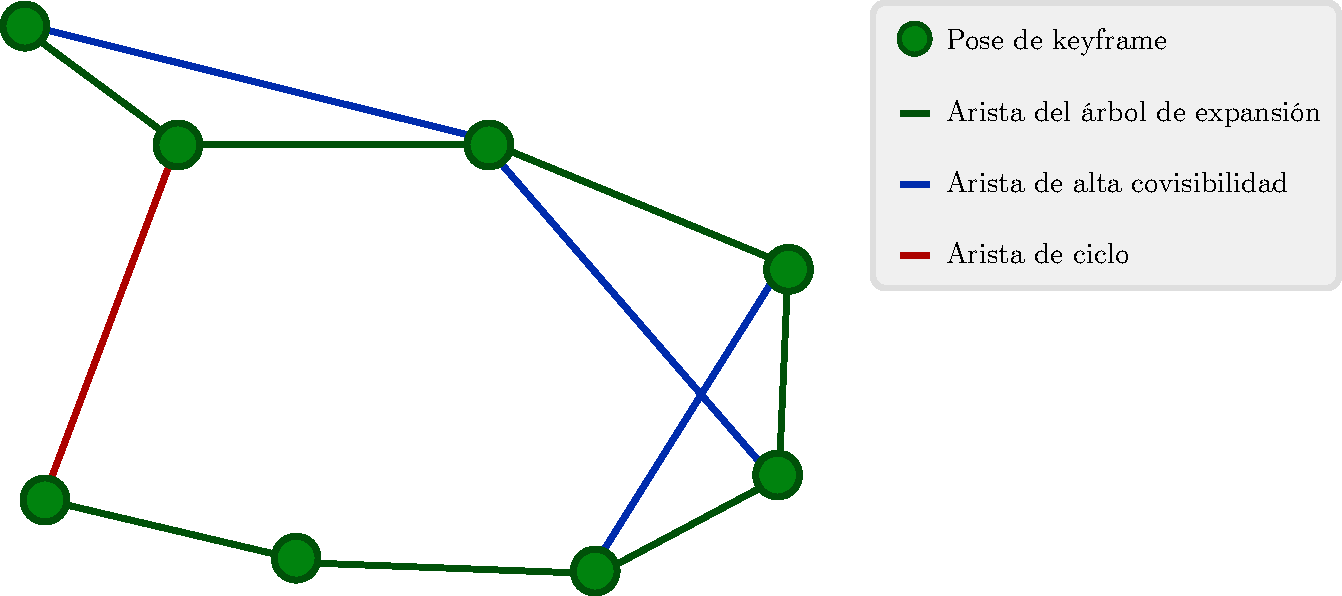
\includegraphics[width=0.4\linewidth]{img/method/pose-graph.pdf}
    \caption{Grafo de poses que se optimiza en PGO.}
    \label{fig:essential_graph}
\end{figure}

Una vez finalizada la optimización, las poses resultantes se devuelven al mapa persistente. A continuación se inicia la etapa de fusión de mapa, descrita en la sección siguiente.

\subsection{Fusión de mapa}

La fusión de mapa se ejecuta como etapa final del proceso, independientemente de si se llevó a cabo una optimización PGO. Comprende tres pasos: aplicar las poses optimizadas, registrar el ciclo en el grafo y fusionar los landmarks correspondientes.

Si se realizó el PGO, se aplican las poses resultantes al mapa mediante \texttt{mergeKeyframesPoses} (Código~\ref{lst:map_merge_opt_poses}). Este método reemplaza las poses del mapa por las optimizadas, incorporando además los keyframes que se hayan introducido entre el momento en que se tomó el snapshot y el fin de la optimización.

\begin{lstlisting}[language=C++, caption={Pseudocódigo del proceso de aplicación de poses optimizadas a los keyframes del mapa.}, label={lst:map_merge_opt_poses}]
template <class Scalar_>
void LandmarkDatabase<Scalar_>::mergeKeyframesPoses(
    std::shared_ptr<Eigen::aligned_map<FrameId, Sophus::SE3<Scalar_>>> optimized_poses) {
  FrameId last_optimized_keyframe = optimized_poses->rbegin()->first;

  // Add the new keyframe poses from keyframe_poses to optimized_poses
  for (auto it = keyframe_poses->upper_bound(last_optimized_keyframe); it != keyframe_poses->end(); ++it) {
    (*optimized_poses)[it->first] = it->second;
  }

  // Replace the pointer to the map poses with the pointer to the new optimized poses
  keyframe_poses = optimized_poses;
}
\end{lstlisting}

A continuación, se registra el ciclo detectado en el grafo de ciclos, agregando una arista que conecta $k_r$ con $k_c$.

Finalmente, se fusionan los landmarks que resultaron inliers durante la verificación geométrica. Para cada correspondencia se presentan dos casos:

\begin{itemize}
    \item El keypoint de $k_r$ no está triangulado. Esto ocurre cuando el front-end lo detectó pero el VIO no pudo triangularlo, o cuando fue agregado durante la proyección de landmarks en la etapa de detección. En ambos casos, se registra una nueva observación del landmark de $k_c$ en $k_r$.
    \item El keypoint de $k_r$ ya está triangulado. Existen entonces dos landmarks con distintos identificadores que representan el mismo punto del mundo. Se fusionan transfiriendo todas las observaciones de uno al otro y eliminando el primero (Código~\ref{lst:map_merge_landmarks}). Se conserva el landmark de $k_r$, dado que puede encontrarse aún en la ventana activa del VIO; de este modo se evita tener que notificarle sobre la fusión.
\end{itemize}

\begin{lstlisting}[language=C++, caption={Pseudocódigo del proceso de fusión de landmarks.}, label={lst:map_merge_landmarks}]
template <class Scalar_>
void LandmarkDatabase<Scalar_>::mergeLandmarks(const LandmarkId& from_lm_id, const LandmarkId& to_lm_id) {
  // The from_lm_id landmark will be merged into the to_lm_id landmark, and then removed from the database.

  if (from_lm_id == to_lm_id) return;

  // Get the landmarks
  auto& from_lm = getLandmark(from_lm_id);
  auto& to_lm = getLandmark(to_lm_id);

  // Merge observations
  for (const auto& [tcid, pos] : from_lm.obs) {
    // Add each observation of the from_lm to the to_lm
  }

  // Remove the from_lm landmark
  removeLandmark(from_lm_id);
}
\end{lstlisting}

Tras cada modificación, ya sea el registro de una nueva observación o la fusión de landmarks, se actualizan las aristas del grafo de covisibilidad para mantenerlo consistente con el estado del mapa.

\section{Mejoras en MapDatabase}

A partir de las funcionalidades implementadas para el cierre de ciclos, fue necesario realizar algunos
ajustes en la clase MapDatabase, que se detallan en esta sección.

\subsection{Reintroducción de keyframes covisibles}

Con la introducción de un grafo de covisibilidad, se habilita la posibilidad de mejorar la eficiencia
de la estrategia de ``Covisibilidad por observaciones'' para resolver las consultas de covisibilidad del VIO.
En primer lugar, se utiliza el grafo de covisibilidad para obtener todos los keyframes covisibles con el
último keyframe introducido, que compartan un mínimo configurable de observaciones. A partir de esto,
se toman los 3 keyframes más viejos y se responde al VIO con estos keyframes junto con todos los landmarks
hosteados por ellos. De esta manera, se obtiene una ventana de covisibilidad más informativa, que
favorece la reintroducción de keyframes que hayan sido candidatos para algún cierre de ciclo junto con
algún keyframe reciente.

A su vez, es importante notar que, con respecto a la estrategia de covisibilidad espacial, surge una
complicación porque la pose de los keyframes en el mapa persistente ya no es estática. Es decir, cada vez
que se realiza alguna optimización sobre las poses de los keyframes, estas cambian, lo que hace que el
cubo de distribución espacial de cada keyframe también cambie. Como cada vez que se optimiza el grafo de poses
todos (a excepción de los keyframes aún activos en la ventana local del VIO) cambian su pose, esto implica
que cada vez que se optimiza el grafo de poses, se deben actualizar todos los cubos de distribución espacial.
Esto no fue implementado porque puede resultar costoso, y se decidió utilizar la estrategia de covisibilidad
por observaciones cuando se habilite el cierre de ciclos. Una posible solución, que queda por fuera del alcance
de este trabajo, sería modificar la manera en que se almacenan y consultan los cubos para que estén definidos
en referencia a la pose del keyframe. De esta manera, aunque la pose del keyframe cambie, el cubo de
distribución espacial se mantendría estático con respecto a la pose del keyframe, y no sería necesario
actualizar todos los cubos cada vez que se optimiza el grafo de poses.

% TODO: poner figura?

\subsection{Culling de keyframes}

Como suele ser el caso de gran parte de los sistemas de SLAM basados en keyframes, el mapa persistente
puede crecer de manera indefinida a medida que se exploran nuevas zonas. Esto trae aparejado un aumento
en el cosumo de recursos del sistema, tanto en memoria como en tiempo de procesamiento. Que el mapa
crezca de manera indefinida es especialmente problemático con el esquema de optimización de ciclos
implementado. En primer lugar, si el mapa contiene un número alto de keyframes, la copia del grafo de
poses que realiza \texttt{MapDatabase} se vuelve cada vez más pesada. Además, como cada vez que se optimiza
el grafo de poses se actualizan las poses de todos los keyframes, contar con un número alto de keyframes
hace que el proceso de PGO se vuelva extremadamente lento. Por estos motivos, se implementó una estrategia
de culling de keyframes, que se encarga de eliminar del mapa persistente aquellos keyframes que resulten
de menor utilidad para el sistema, manteniendo el mapa acotado en tamaño.

Cuando se decide eliminar un keyframe, se elimina su pose, todos los landmarks que hosteaba, todas las
referencias a ese keyframe en el \texttt{CovisibilityGraph} y todas las observaciones, actualizando el
grafo de covisibilidad para mantenerlo consistente con la información del mapa.

En primer lugar, y de manera similar al esquema de culling de keyframes que utiliza ORB-SLAM3,
cada vez que se marginaliza un keyframe en el VIO, \texttt{MapDatabase} calcula el porcentaje de landmarks,
de todas las que observa el keyframe marginalizado, que son observadas por al menos otros 3 keyframes
del mapa. Si este porcentaje es menor al 90\% se retiene el keyframe. De lo contrario, se elimina del
mapa. Eso permite eliminar de manera temprana aquellos keyframes cuya redundancia es tan alta que no
aportan información relevante para el sistema. Este mecanismo suele eliminar keyframes principalmente
cuando las cámaras se encuentran estáticas, observando la misma escena. 

Además, se implementa también una estrategia de culling de keyframes más agresiva, que establece un número
máximo de keyframes que el mapa puede contener, y cada vez que se supera ese número, se eliminan
keyframes en batches. Para esto, se definen heurísticas para establecer un puntaje de utilidad de cada
keyframe, y se eliminan aquellos con menor puntaje. Se añade un atributo denominado \texttt{keyframe\_scores}
a la clase \texttt{MapDatabase} para almacenarlos, cuyo detalle se muestra en el Código 5.7.
Este puntaje se calcula a partir de una suma pesada
de diferentes factores que se muestran a continuación:

$$ score(k) = 0.4 * S_g + 0.2 * S_l + 0.1 * S_t + 0.1 * S_c + 0.2 * S_o $$

donde:

\begin{itemize}
    \item Cantidad de landmarks observados ($S_o$): Un keyframe que observa pocos landmarks (menos
    de 10 por ejemplo) es de una calidad baja. Incluso es probable que su pose tenga mucho error.
    Pero, al mismo tiempo, un keyframe con una gran cantidad de landmarks observados no necesariamente
    es bueno para mantenerlo, porque probablemente observe lo mismo que otros keyframes y se vuelva redundante.
    La intención de este score es penalizar los primeros (los keyframes con muy pocos landmarks)
    sin favorecer los que tengan muchos. De esta manera, se elige la función $\frac{x}{x+10}$. La diferencia
    entre los números bajos implica un cambio mayor en el score, pero no en los números más altos (tiene
    derivada decreciente).
    Este puntaje se calcula solo una vez, cuando el keyframe es marginalizado.
    \item Cubrimiento de las imágenes del frame ($S_c$):
    Un keyframe que observa puntos solo en una parte de la imagen podría ser de menor calidad que uno que
    los observa en más partes. Para esto, se calcula el \textit{bounding box} que contenga a todas las
    observaciones para cada cámara y se calcula el ratio del área en comparación con el tamaño de la imagen.
    Finalmente, se calcula el promedio del ratio de todas las cámaras del keyframe.
    Este puntaje se calcula solo una vez, cuando el keyframe es marginalizado.
    \item Utilidad temporal ($S_t$):
    Los keyframes más viejos tienen utilidad porque son los que menos drift contienen (o uno esperaría que
    esto fuera así). Los más nuevos son de utilidad porque corresponden a la escena que actualmente está
    siendo mapeada. Entonces, se elige un score que penalice a los keyframes de la mitad. Se elige la
    función con forma de ``V'' $|2x-1|$. Dado que esto está basado más en una intuición que en un valor
    real, su peso es bajo.
    Este puntaje se calcula cada vez que se supera el número máximo de keyframes, para todos los
    keyframes del mapa.
    \item Reemplazabilidad en el grafo de covisibilidad ($S_g$):
    La intuición es que un keyframes es reemplazable si al eliminarlo se mantiene la misma estructura en
    el grafo de covisibilidad. Por ejemplo, un keyframe que hace una especie de ``puente'' entre dos
    componentes conexas no se debería eliminar. Para aproximar esta idea, se utiliza la cantidad de
    aristas de alta covisibilidad incidentes en el nodo (grado de alta covisibilidad).
    Se utiliza la función $1 - \min(x/10,1)$ donde $x$ es el grado de alta covisibilidad del keyframe.
    Cada vez que se agrega o elimina una arista de alta covisibilidad que incida en el nodo del keyframe,
    la clase \texttt{CovisibilityGraph} actualiza el puntaje de reemplazabilidad de los keyframes afectados,
    y se notifica a \texttt{MapDatabase} para que actualice el puntaje total de cada keyframe afectado
    mediante un callback.
    \item Cantidad de detecciones de ciclo ($S_l$):
    Si un nodo se usó para varios loop closures, entonces es probable que ese nodo sea importante para la
    consistencia global del mapa. Se debería subir el score considerablemente incluso con 1 loop closure.
    Se utiliza la función $\frac{x}{x+1}$ donde $x$ es el número de loop closures en los cuales estuvo involucrado
    el keyframe.
    Cada vez que se agrega una arista de ciclo que incida en el nodo del keyframe, la clase
    \texttt{CovisibilityGraph} actualiza el puntaje de cantidad de detecciones de ciclo de los keyframes
    afectados, y se notifica a \texttt{MapDatabase} para que actualice el puntaje total de cada keyframe afectado
    mediante un callback.
\end{itemize}

\begin{figure}[ht]
    \centering
    \begin{subfigure}[b]{0.32\textwidth}
        \centering
        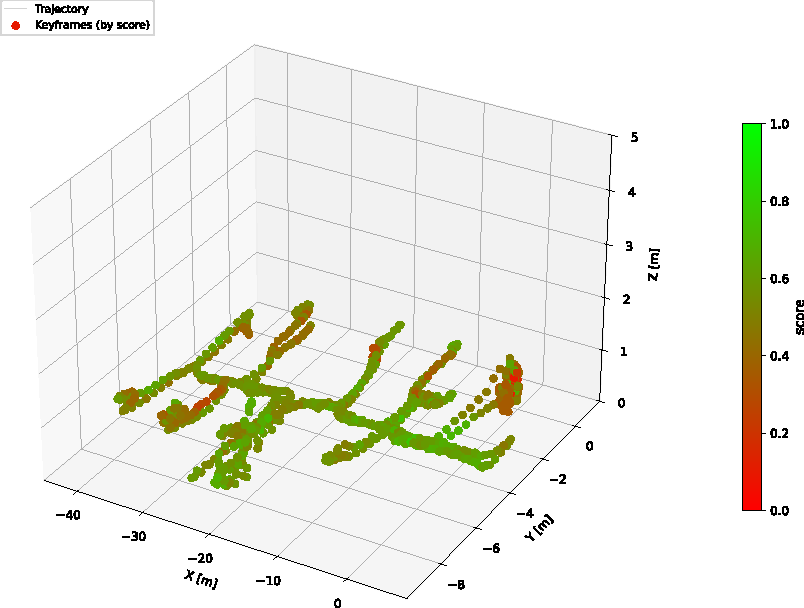
\includegraphics[width=\textwidth]{img/method/scores.pdf}
        \caption{Weighted scores}
        \label{fig:weighted_scores}
    \end{subfigure}
    \hfill
    \begin{subfigure}[b]{0.32\textwidth}
        \centering
        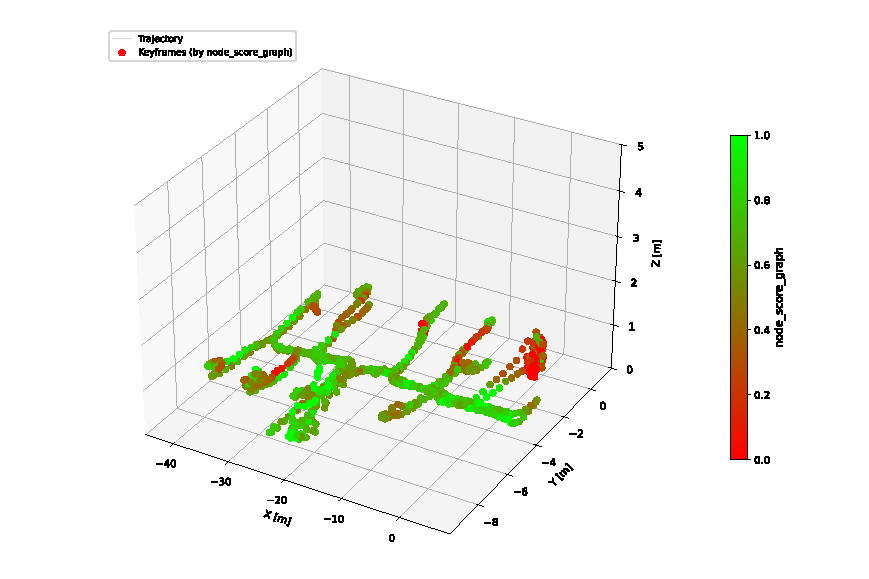
\includegraphics[width=\textwidth]{img/method/score-node-graph.pdf}
        \caption{Degree of high covisibility edges score}
        \label{fig:score_node_graph}
    \end{subfigure}
    \hfill
    \begin{subfigure}[b]{0.32\textwidth}
        \centering
        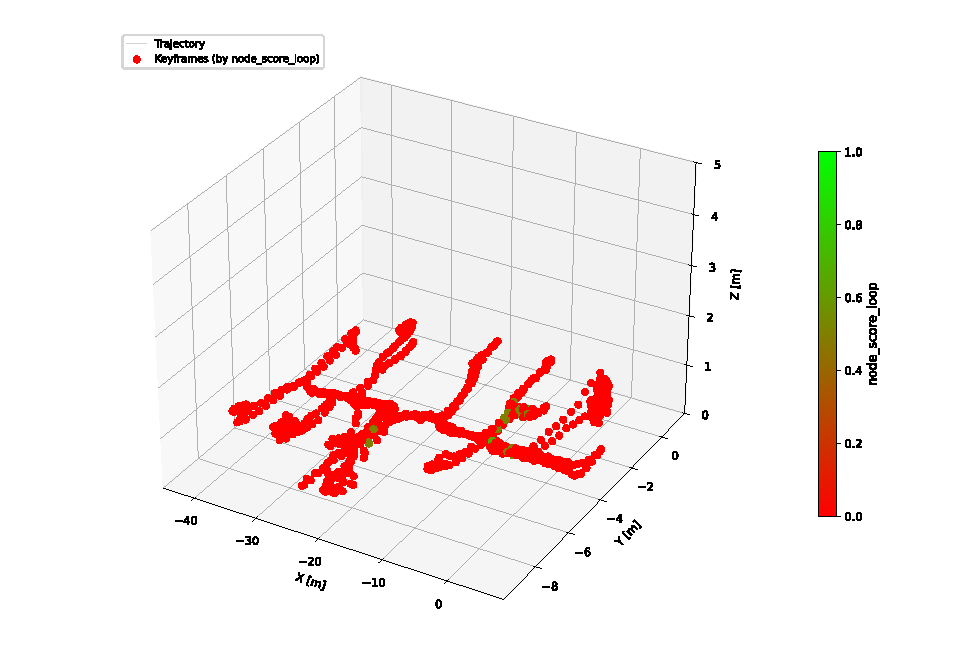
\includegraphics[width=\textwidth]{img/method/score-node-loop.pdf}
        \caption{Degree of loop closure edges score}
        \label{fig:score_node_loop}
    \end{subfigure}

    \vspace{0.5em}

    \begin{subfigure}[b]{0.32\textwidth}
        \centering
        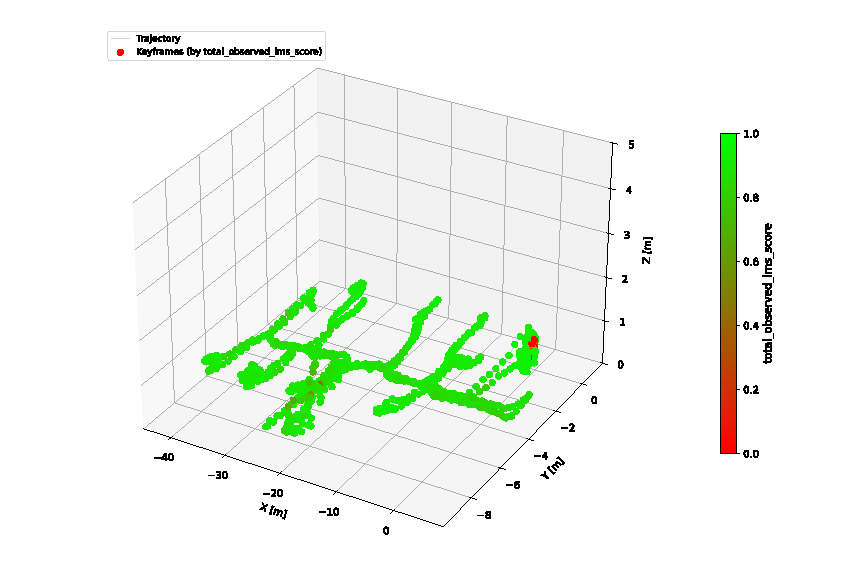
\includegraphics[width=\textwidth]{img/method/score-obs.pdf}
        \caption{Number of observed landmarks score}
        \label{fig:score_obs}
    \end{subfigure}
    \hfill
    \begin{subfigure}[b]{0.32\textwidth}
        \centering
        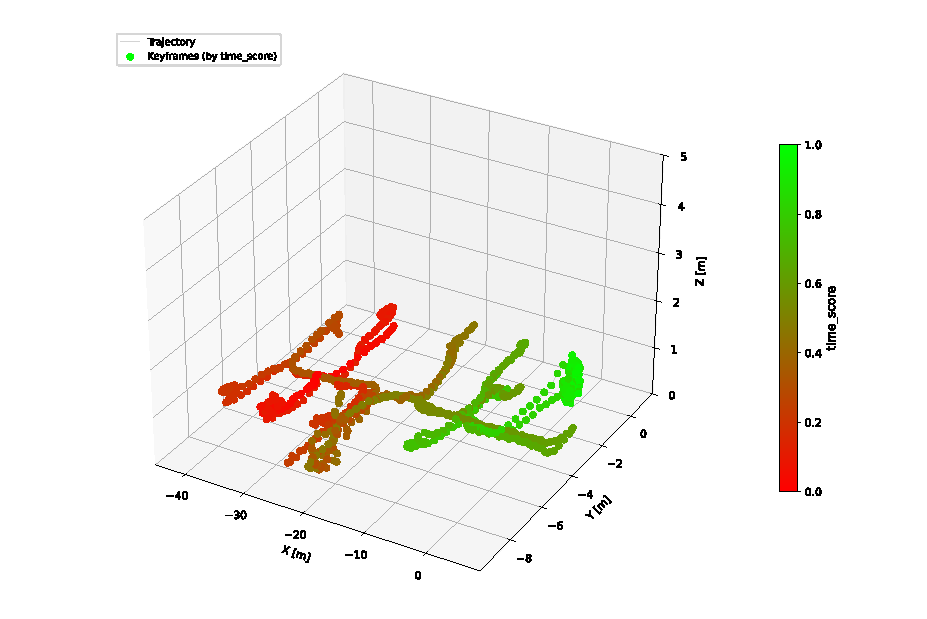
\includegraphics[width=\textwidth]{img/method/score-times.pdf}
        \caption{Time-based score}
        \label{fig:score_times}
    \end{subfigure}
    \hfill
    \begin{subfigure}[b]{0.32\textwidth}
        \centering
        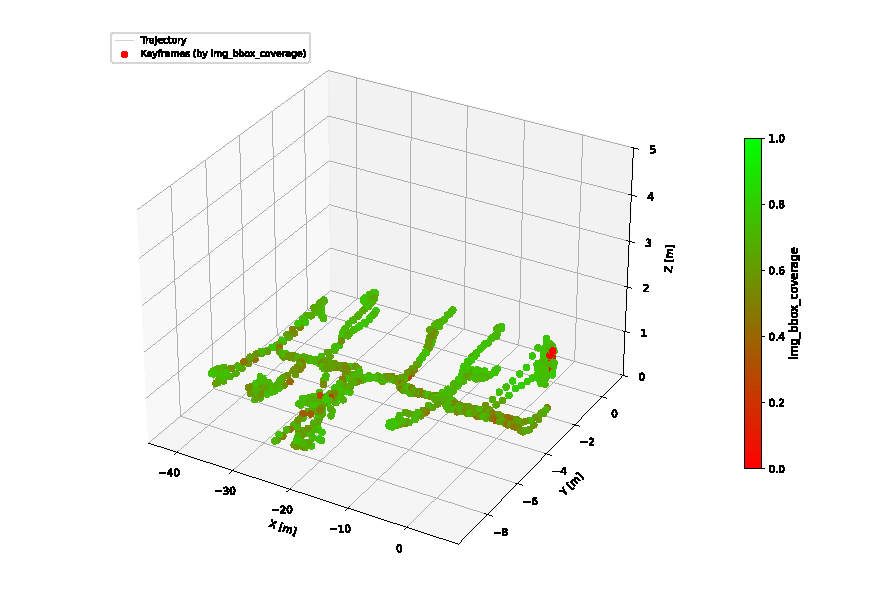
\includegraphics[width=\textwidth]{img/method/score-bbox.pdf}
        \caption{Bounding box score}
        \label{fig:score_bbox}
    \end{subfigure}

    \caption{Comparativa de los diferentes factores que componen el puntaje de utilidad de cada keyframe.}
    \label{fig:keyframe_scores}
\end{figure}

% TODO: este diagrama no va aca. aca hacer un diagrama que muestre la idea
% esa figura va en experimentacion

% primero mostrar figuras, y después poner el texto, asi ya lo leen con la idea en mente

% se tuvo que bajar este valor. sin dudas este proceso de culling de keyframes es un área que se podría
% mejorar, y al menos tunear estos parámetros y pesos mejor.
% loop_closing_pgo_min_covisibility_weight = 60

Mediante esta estrategia, se establece un límite máximo de 1500 keyframes en el mapa persistente,
y cada vez que \texttt{MapDatabase} recibe un nuevo \texttt{MapStamp} del VIO que hace que el número
de keyframes supere ese límite, se eliminan los 30 keyframes con menor puntaje.

\subsection{Interfaz final del mapa persistente}

% por ahí lo puedo mandar al apendice

Toda la comunicación que se dirija al mapa persistente, pasa por una de las dos colas de trabajo
disponibles: \texttt{read\_queue} y \texttt{write\_queue}. Dada la variedad de mensajes que pueden
recibir, se definen tipos variante para cada una de las colas, como se muestra en el Código
\ref{lst:map_message_types}.

\begin{lstlisting}[language=C++, caption={Definición de los tipos de mensajes aceptados por las colas de lectura y escritura del mapa persistente.}, label={lst:map_message_types}]
using MapWriteMessage = std::variant<MapStamp::Ptr,
                                     MarginalizationStamp::Ptr,
                                     LoopDetectionResult::Ptr,
                                     LoopClosureResult::Ptr,
                                     StopMsg>;

using MapReadMessage = std::variant<CovisibilityRequest::Ptr,
                                    IslandRequest::Ptr,
                                    StopMsg>;
\end{lstlisting}


Luego, cada thread del mapa persistente se implementa como se muestra en el Código \ref{lst:map_read_thread}
y \ref{lst:map_write_thread}.

\begin{lstlisting}[language=C++, caption={Pseudocódigo del thread de lectura del mapa persistente.}, label={lst:map_read_thread}]
MapReadMessage msg;
bool running = true;

while (running) {
    read_queue.pop(msg);

    std::visit(
        [&](auto& m) {
        using T = std::decay_t<decltype(m)>;

        if constexpr (std::is_same_v<T, CovisibilityRequest::Ptr>) {
            read_covisibility_req(m->keypoints);
        } else if constexpr (std::is_same_v<T, IslandRequest::Ptr>) {
            read_island_req(m->keyframe, m->num_neighbors);
        } else if constexpr (std::is_same_v<T, StopMsg>) {
            // Send termination signals
            running = false;
        }
        },
        msg);
}
\end{lstlisting}

\begin{lstlisting}[language=C++, caption={Pseudocódigo del thread de escritura del mapa persistente.}, label={lst:map_write_thread}]
MapWriteMessage msg;

bool running = true;
while (running) {
    write_queue.pop(msg);

    std::visit(
        [&](auto& m) {
        using T = std::decay_t<decltype(m)>;

        if constexpr (std::is_same_v<T, MapStamp::Ptr>) {
            write_map_stamp(m);
        } else if constexpr (std::is_same_v<T, MarginalizationStamp::Ptr>) {
            write_map_marg(m->keyframe_ids);
        } else if constexpr (std::is_same_v<T, LoopDetectionResult::Ptr>) {
            handle_loop_detection(m);
        } else if constexpr (std::is_same_v<T, LoopClosureResult::Ptr>) {
            handle_loop_closure(m);
        } else if constexpr (std::is_same_v<T, StopMsg>) {
            // Send termination signals and save the map if necessary
            running = false;
        }
        },
        msg);
}
\end{lstlisting}

\section{RootBA para un sistema de SLAM}

% TODO: agregar figuras del paper de las JAR

RootBA es un método de Bundle Adjustment a gran escala cuya implementación propuesta se adapta
al contexto de \textit{Structure From Motion} (SfM). Su implementación se encuentra disponible en \href{https://github.com/nikolausdemmel/rootba}. Para adaptarla al contexto de un sistema de SLAM, se realizaron algunas modificaciones que se describen en esta sección.

\subsection{Eliminación de parámetros intrínsecos del estado}

En primer lugar, al ser un método de SfM, el algoritmo no solo estima poses de cámaras y posiciones de puntos 3d, si no que también estima los parámetros intrínsecos de las cámaras. Utiliza el modelo de cámara utilizado en el Paper "Bundle Adjustment in the Large", con 6 parámetros extrínsecos y 3 intrínsecos: distancia focal $f$ y 2 parámetros de distorsión radial $k_1$ y $k_2$. Esto es útil en métodos de SfM, donde el conjunto de imágenes puede provenir de distintos orígenes, inlcuso cada una puede haber sido tomada por una cámara distinta. En el contexto de SLAM para XR, donde las calibraciones de las cámaras son conocidas y, más aún, todas las imágenes provienen de las mismas cámaras, ya no tiene sentido optimizar los parámetros intrínsecos de las cámaras. Además, considerar que todas las imágenes pueden provenir de cámaras distintas puede causar que, en vez de corregir el error de una pose de una cámara, se compence modificando algún valor de distorsión de su calibración.

Para corregir esto, simplemente se eliminan las variables relacionadas a los parámetros intrínsecos de las cámaras del vector de estado. Luego, no se computan ni almacenen las derivadas relacionadas a estos parámetros en los Landmark Blocks, como se observa en la Figura \ref{fig:rootba-intrinsics}.

\subsection{Optimización de poses de rigs}

Una característica del sistema propuesto es que las imágenes capturadas por
las múltiples cámaras de un mismo keyframe comparten una transformación
relativa conocida entre sí, constante a lo largo de todos los keyframes.
Si se tratara a todas las cámaras como variables independientes en el vector
de estado, la optimización podría romper esta restricción de rigidez entre
las cámaras del rig.

Para remediar esto, en lugar de almacenar las poses de cada cámara
individualmente, se almacena la pose de la IMU como representación del
rig completo en cada instante de tiempo. Este cambio de variables implica
modificar el algoritmo de linealización, de modo que los incrementos
calculados correspondan a perturbaciones sobre la pose del \emph{body}.

Sean $T_b \in SE(3)$ la pose del body y $T_c \in SE(3)$ la pose de una
cámara del rig en el mismo instante de tiempo. La transformación relativa
entre ambos es fija y conocida, dada por la calibración extrínseca
$T_{cb} \in SE(3)$:
\begin{equation}
    T_c = T_{cb} \cdot T_b.
    \label{eq:rig_composition}
\end{equation}

Con la parametrización propuesta, en lugar de $\frac{\partial r}{\partial \Delta x_c}$
se requiere $\frac{\partial r}{\partial \Delta x_b}$. Por \eqref{eq:adjoint_twist}, la perturbación sobre la cámara se relaciona con
la del body mediante $\Delta x_c = \mathrm{Ad}_{T_{cb}}\,\Delta x_b$, de donde:
\begin{equation}
    \frac{\partial\,\Delta x_c}{\partial\,\Delta x_b} = \mathrm{Ad}_{T_{cb}}.
    \label{eq:jacobian_deltax}
\end{equation}
Aplicando la regla de la cadena:
\begin{equation}
    \frac{\partial r}{\partial \Delta x_b}
    = \frac{\partial r}{\partial \Delta x_c}
      \cdot \mathrm{Ad}_{T_{cb}}.
    \label{eq:chain_rule_result}
\end{equation}

Además, otra diferencia es que ahora, cada landmark puede afectar la pose de un rig mediante más de una observación, pues hay múltiples cámaras asociadas a un mismo rig, que pueden aportar observaciones del mismo landmark. Estas modificaciones pueden observarse en la Figura \ref{fig:rootba-rigs}.

\begin{figure}[h]
    \centering
    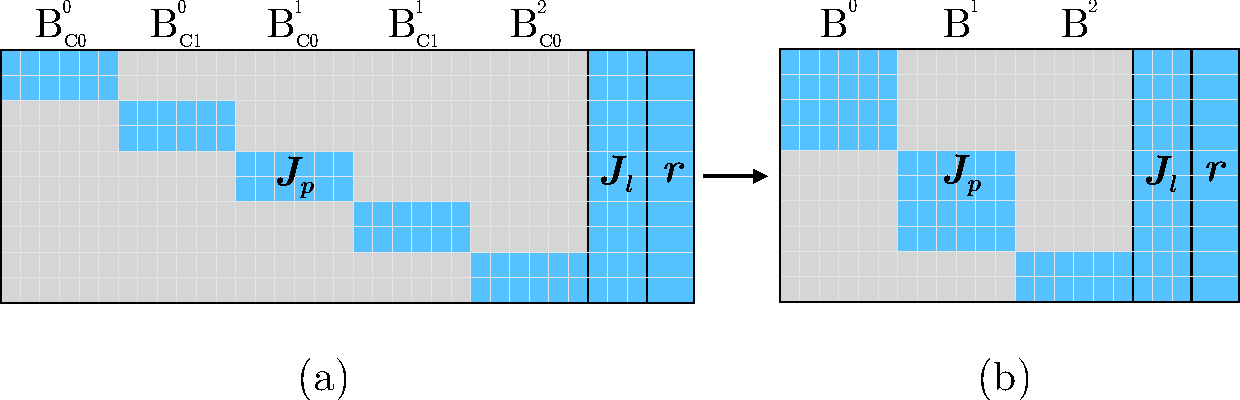
\includegraphics[width=0.8\linewidth]{img/method/rootba-rigs.pdf}
    \caption{Representación de rigs en el estado de rootba.}
    \label{fig:rootba-rigs}
\end{figure}

% TODO: skip de kfs con pocas obs??
